% MapOSMatic - Libre Software Meeting 2012 presentation
% -*- coding: utf-8; mode: LaTeX -*-

% Copyright (C) 2010 Maxime Petazzoni <maxime.petazzoni@bulix.org>
%                    Thomas Petazzoni <thomas.petazzoni@enix.org>
% Distributed under the terms of the Creative Commons CC-by-sa 3.0

\documentclass{beamer}
\usepackage[utf8]{inputenc}
\usepackage[american]{babel}

\mode<presentation>
\usetheme{MapOSMatic}
\setbeamercovered{dynamic}

\title{MapOSMatic: city maps for the masses}
\author{Thomas {\sc Petazzoni}}
\institute{Libre Software Meeting}
\date{July 10th, 2012}

\begin{document}

%%%%%%%%%%%%%%%%%%%%%%%%%%%%%%%%%%%%%%%%%%%%%%%%%%%%%%%%%%%%%%%%%%%%%%%

\begin{frame}
  \titlepage
\end{frame}

\begin{frame}{Thomas Petazzoni}
  \begin{itemize}
  \item {\bf Embedded Linux engineer} and trainer at Free Electrons
  \item Regular contributor to the {\bf Buildroot} project, an open-source
    embedded Linux build system
  \item Contributor to the Linux {\bf kernel}
  \item Active in the free software community: founder of {\em
      Toulibre}, founder of the {\em Agenda du Libre}
  \item {\bf One of the developer of MapOSMatic}, together with
    David Decotigny, Gaël Utard, Maxime Petazzoni, David Mentré,
    Frédéric Lehobey, Étienne Loks, and many other contributors.
  \end{itemize}
\end{frame}

\begin{frame}{Agenda}
  \begin{enumerate}
  \item Original idea and goal
  \item History
  \item Current status
  \item Technical details
  \item Future
  \end{enumerate}
\end{frame}

\begin{frame}{Original idea}
  At some point in 2009...
  \vspace{1cm}
  \\
  \Large
  \begin{quote}
    ``It would be great to be able to use OpenStreetMap data to generate
    city maps such as the ones we can see in town signs and in folded
    maps.''
  \end{quote}
  \normalsize
  \vspace{1cm}
  \hfill Gilles Lamiral, OSM contributor of Bretagne, France
\end{frame}

\begin{frame}{Public city maps}
  \begin{center}
    \includegraphics[height=0.8\textheight]{public-city-map.jpg}
  \end{center}
\end{frame}

\begin{frame}{Folded maps}
  \begin{center}
    \includegraphics[height=0.8\textheight]{folded-map.jpg}
  \end{center}
\end{frame}

\begin{frame}{Goal}
  \Large
  Create an {\bf easy-to-use Web service}, in which the user inputs
  the {\bf name of a city}, and in return gets:
  \begin{enumerate}
  \item a {\bf map} of that city, overlayed by a {\bf grid}
  \item an {\bf index of streets and amenities} associated to the map
  \end{enumerate}
\end{frame}

\begin{frame}{Development model}
  \begin{itemize}
  \item The development mainly takes place during {\bf hackfests}
  \item Hackfests are gathering of 4-6 developers for 2 to 8 days,
    fully dedicated to making progress on the project
  \item Hackfests provide an excellent productivity
  \item Maintenance and minor progress (bug fixes, translation
    updates) done outside of the hackfests, as a regular open-source
    project, with mailing-list, Git repositories, etc.
  \end{itemize}
\end{frame}

\begin{frame}{Hackfest \#0}
  \begin{itemize}
  \item August 2009, Toulouse, France
  \item Six OSM contributors
  \item No knowledge of PostgreSQL, PostGIS, Mapnik, OSM data
    structure, Cairo
  \item Initial version of MapOSMatic developed and published in 5 days
    \begin{itemize}
    \item Technologies: Python, Django, Cairo, PostgreSQL, PostGIS, Mapnik
    \end{itemize}
  \item Limited to France, no support for languages other than French
    and English, very basic user interface, OSM data never updated
  \item \url{http://www.maposmatic.org}
  \item Excellent reception from the OpenStreetMap community
  \end{itemize}
\end{frame}

\begin{frame}{Hackfest \#0 results}
  \begin{center}
    \includegraphics[height=0.8\textheight]{chavagne.png}
    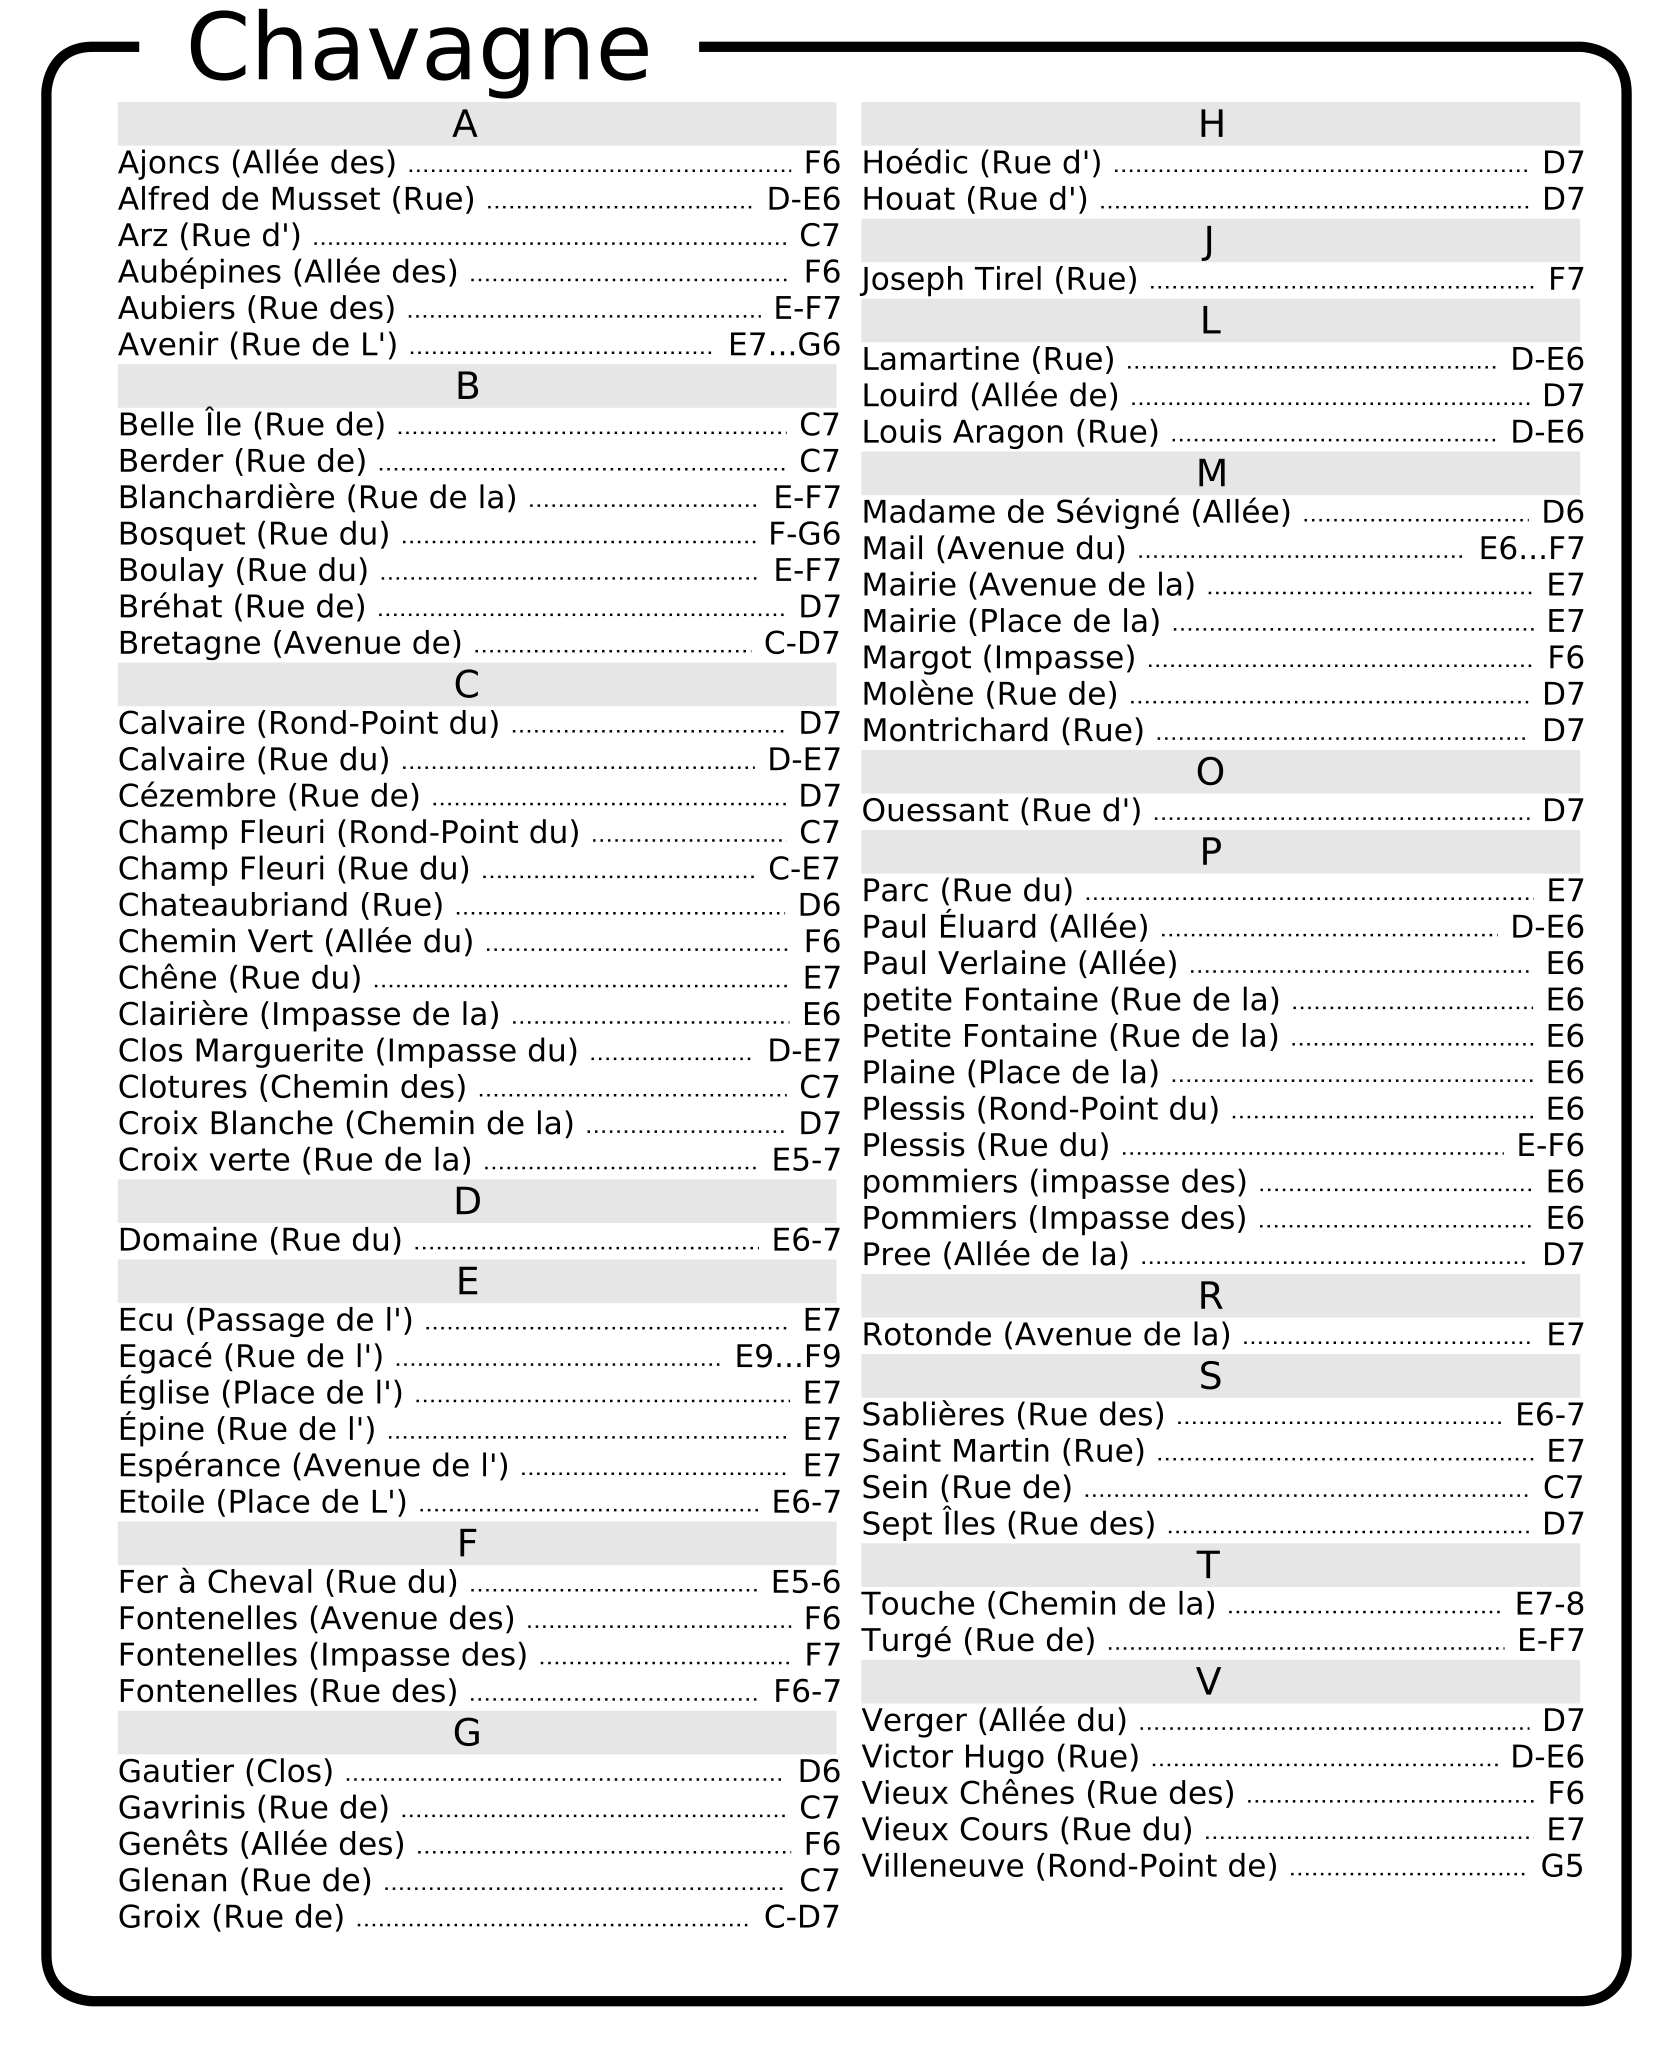
\includegraphics[height=0.8\textheight]{chavagne_index.png}
  \end{center}
\end{frame}

\begin{frame}{Hackfest \#0 details}
  \begin{center}
    \includegraphics[height=0.5\textheight]{chavagne_detail.png}
    \includegraphics[height=0.5\textheight]{chavagne_index_detail.png}
  \end{center}
\end{frame}

\begin{frame}{Hackfest \#1}
  \begin{itemize}
  \item December 2009, near Paris, France
  \item Five developers, four days
  \item Features implemented
    \begin{itemize}
    \item Coverage of the whole world: required a much larger import
      of OSM data
    \item OSM database updated on a daily basis
    \item i18 infrastructure to adapt the street index generation on a
      per-language basis
    \item City name search based on Nominatim
    \item Amenities (schools, town hall, post offices) in the index
    \end{itemize}
  \item All improvements put in production early January 2010
  \item After this hackfest, we started receiving a lot of
    contributions to translate the language and the street index
    rendering logic.
  \end{itemize}
\end{frame}

\begin{frame}{Hackfest \#2}
  \begin{columns}
    \column{0.7\textwidth}
  \begin{itemize}
  \item August 2010, Toulouse, France
  \item Six developers, seven days
  \item Features
    \begin{itemize}
    \item Complete rewrite of the rendering engine, to support
      multiple layouts (index on the same side as the map, at the
      bottom or on the side) and selectable standard paper sizes
    \item Support for multiple stylesheets (style of renderings)
    \item Major rewrite of the web interface, to provide a wizard for
      the map creation
    \end{itemize}
  \item Features not completed, so no delivery in production...
  \end{itemize}
  \column{0.3\textwidth}
  \includegraphics[height=0.5\textheight]{hackfest-2-notes.jpg}
  \end{columns}
\end{frame}

\begin{frame}{Hackfest \#2 result}
  \begin{center}
    \includegraphics[height=0.8\textheight]{stains.png}
  \end{center}
\end{frame}

\begin{frame}{Server migration, october 2010}
  Our initial server, having 250 GB of hard disk space, was completely
  filled with the OpenStreetMap database.\\

  Had to migrate all our services on different machines, causing a
  severe downtime for the service.
\end{frame}

\begin{frame}{Hackfest \#3}
  \begin{columns}
    \column{0.6\textwidth}
  \begin{itemize}
  \item February 2012, San Francisco, USA
  \item Four developers, two days
  \item Things done
    \begin{itemize}
    \item Investigation of a Mapnik rendering bug that was a block for
      releasing in production our new version
    \item Add some monitoring tools on our servers
    \item Polish web interface details
    \end{itemize}
  \item Improvements made in August 2010 were still not in production!
  \end{itemize}
    \column{0.4\textwidth}
  \includegraphics[width=0.9\textwidth]{hackfest-3.jpg}
  \end{columns}
\end{frame}

\begin{frame}{Hackfest \#4}
  \begin{columns}
    \column{0.6\textwidth}
  \begin{itemize}
  \item March 2012, Rennes, France
  \item Five developers, seven days
  \item Objective: put in production all the new features
    \begin{itemize}
    \item Support for multi-page maps, which allows to render large
      maps on A4 and A5 paper sizes
    \item Integration of several Mapnik stylesheets
    \item Many, many fixes in the rendering engine and the web
      interface
    \end{itemize}
  \item {\bf On April, 19th, a few weeks after the hackfest, we
      managed to put all the improvements in production and make it
      public!}
  \end{itemize}
    \column{0.4\textwidth}
  \includegraphics[width=0.9\textwidth]{hackfest-4.jpg}
  \end{columns}
\end{frame}

\begin{frame}{Hackfest \#4 results}
  \begin{center}
    \includegraphics[height=0.8\textheight]{chavagne-multi-page-front.png}
    \includegraphics[height=0.8\textheight]{chavagne-multi-page-overview.png}
  \end{center}
\end{frame}

\begin{frame}{Using maposmatic.org (1/11)}
  \begin{center}
    \includegraphics[width=\textwidth]{screenshot1.png}
  \end{center}
\end{frame}

\begin{frame}{Using maposmatic.org (2/11)}
  \begin{center}
    \includegraphics[width=\textwidth]{screenshot2.png}
  \end{center}
\end{frame}

\begin{frame}{Using maposmatic.org (3/11)}
  \begin{center}
    \includegraphics[width=\textwidth]{screenshot3.png}
  \end{center}
\end{frame}

\begin{frame}{Using maposmatic.org (4/11)}
  \begin{center}
    \includegraphics[width=\textwidth]{screenshot4.png}
  \end{center}
\end{frame}

\begin{frame}{Using maposmatic.org (5/11)}
  \begin{center}
    \includegraphics[width=\textwidth]{screenshot5.png}
  \end{center}
\end{frame}

\begin{frame}{Using maposmatic.org (6/11)}
  \begin{center}
    \includegraphics[width=\textwidth]{screenshot6.png}
  \end{center}
\end{frame}

\begin{frame}{Using maposmatic.org (7/11)}
  \begin{center}
    \includegraphics[width=\textwidth]{screenshot7.png}
  \end{center}
\end{frame}

\begin{frame}{Using maposmatic.org (8/11)}
  \begin{center}
    \includegraphics[width=\textwidth]{screenshot8.png}
  \end{center}
\end{frame}

\begin{frame}{Using maposmatic.org (9/11)}
  \begin{center}
    \includegraphics[width=\textwidth]{screenshot9.png}
  \end{center}
\end{frame}

\begin{frame}{Using maposmatic.org (10/11)}
  \begin{center}
    \includegraphics[width=\textwidth]{screenshot10.png}
  \end{center}
\end{frame}

\begin{frame}{Using maposmatic.org (11/11)}
  \begin{center}
    \includegraphics[width=\textwidth]{screenshot11.png}
  \end{center}
\end{frame}

\begin{frame}{OSM Database}

\end{frame}

\begin{frame}{OCitySMap}

\end{frame}

\begin{frame}{MapOSMatic}

\end{frame}

\begin{frame}{Hardware setup}

\end{frame}

\begin{frame}{Statistics}

\end{frame}

\begin{frame}{Examples of usage}

\end{frame}

\begin{frame}[t]{Conclusion}
\end{frame}

\end{document}
